\documentclass[tikz,border=10pt]{standalone}
\usepackage{amsmath}
\usepackage[T1]{fontenc}
\usepackage{tikz}
\usetikzlibrary{positioning,arrows.meta,backgrounds,fit,calc,matrix}

% =====================================================================
%  Convolución 2D  (2D convolution illustration)
%  Standalone, compilable. To embed in the thesis copy the
%  \begin{tikzpicture}...\end{tikzpicture} block into a figure and
%  load in the preamble:
%     \usetikzlibrary{positioning,arrows.meta,backgrounds,fit,calc,matrix}
% =====================================================================

\definecolor{cblue}{RGB}{31,90,150}
\definecolor{cbluefill}{RGB}{225,236,247}
\definecolor{cgreen}{RGB}{40,120,55}
\definecolor{cgreenfill}{RGB}{231,243,228}
\definecolor{cpurple}{RGB}{95,50,135}
\definecolor{cpurplefill}{RGB}{240,235,247}
\definecolor{cnavy}{RGB}{20,45,90}

\begin{document}
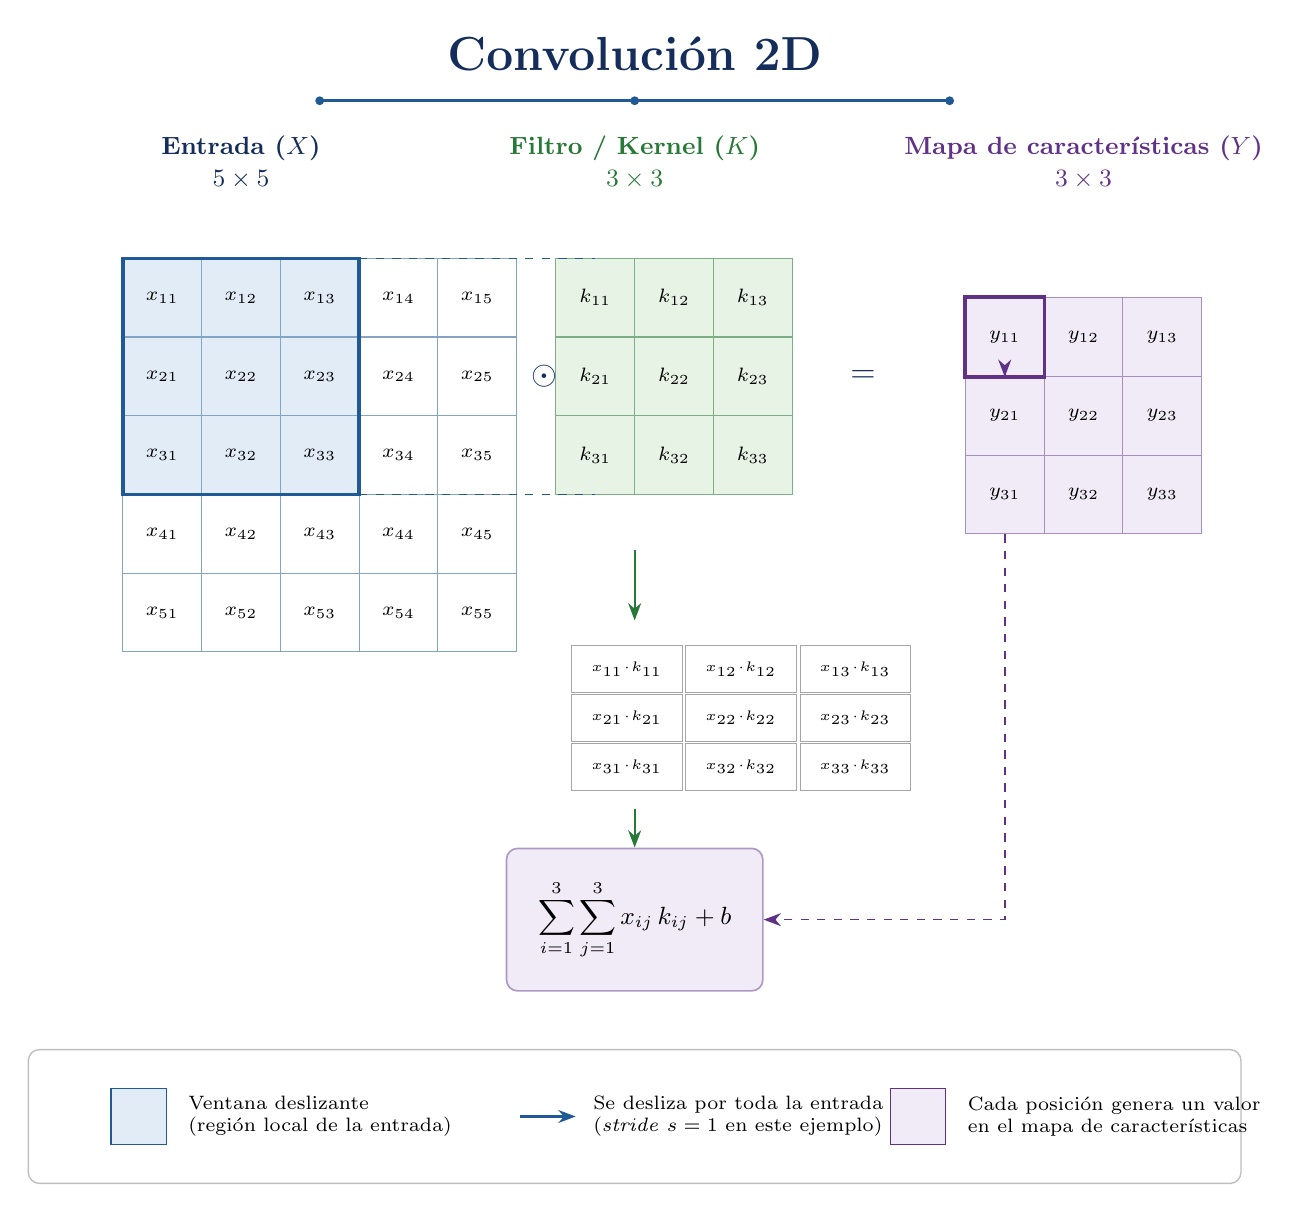
\begin{tikzpicture}[
  font=\small,
  cell/.style={minimum size=10mm, draw=cblue!55, line width=0.4pt, anchor=center},
  >={Stealth[length=2.2mm]}
]

% TITLE
\node[cnavy] at (7.0,4.6) {\bfseries\LARGE Convolución 2D};
\draw[cblue, line width=1pt] (3.0,4.0)--(11.0,4.0);
\fill[cblue] (3.0,4.0) circle (1.6pt); \fill[cblue] (7.0,4.0) circle (1.6pt); \fill[cblue] (11.0,4.0) circle (1.6pt);

% INPUT 5x5
\node[cnavy] at (2.0,3.4) {\bfseries Entrada ($X$)};
\node[cnavy] at (2.0,3.0) {$5\times5$};
\begin{scope}[on background layer]
  \fill[cbluefill] (0.5,2.0) rectangle (3.5,-1.0);
\end{scope}
\foreach \r in {1,...,5}{
  \foreach \c in {1,...,5}{
    \pgfmathtruncatemacro{\rr}{\r}
    \pgfmathtruncatemacro{\cc}{\c}
    \node[cell] (X\r\c) at ({\c*1.0},{2.5-\r*1.0}) {\scriptsize$x_{\rr\cc}$};
  }
}
\draw[cblue, line width=1.2pt] (0.5,2.0) rectangle (3.5,-1.0);

% KERNEL 3x3
\node[cgreen] at (7.0,3.4) {\bfseries Filtro / Kernel ($K$)};
\node[cgreen] at (7.0,3.0) {$3\times3$};
\foreach \r in {1,...,3}{
  \foreach \c in {1,...,3}{
    \pgfmathtruncatemacro{\rr}{\r}
    \pgfmathtruncatemacro{\cc}{\c}
    \node[cell, draw=cgreen!60, fill=cgreenfill] (K\r\c) at ({5.5+\c*1.0},{2.5-\r*1.0}) {\scriptsize$k_{\rr\cc}$};
  }
}

\node[cnavy] at (5.85,0.5) {\large $\odot$};
\node[cnavy] at (9.9,0.5) {\large $=$};

\draw[cblue, dashed, line width=0.4pt] (3.5,2.0)--(6.5,2.0);
\draw[cblue, dashed, line width=0.4pt] (3.5,-1.0)--(6.5,-1.0);

% OUTPUT 3x3
\node[cpurple] at (12.7,3.4) {\bfseries Mapa de características ($Y$)};
\node[cpurple] at (12.7,3.0) {$3\times3$};
\foreach \r in {1,...,3}{
  \foreach \c in {1,...,3}{
    \pgfmathtruncatemacro{\rr}{\r}
    \pgfmathtruncatemacro{\cc}{\c}
    \node[cell, draw=cpurple!55, fill=cpurplefill] (Y\r\c) at ({10.7+\c*1.0},{2.0-\r*1.0}) {\scriptsize$y_{\rr\cc}$};
  }
}
\draw[cpurple, line width=1.3pt] (Y11.south west) rectangle (Y11.north east);

% ELEMENTWISE PRODUCT GRID
\foreach \r in {1,...,3}{
  \foreach \c in {1,...,3}{
    \pgfmathtruncatemacro{\rr}{\r}
    \pgfmathtruncatemacro{\cc}{\c}
    \node[draw=black!35, line width=0.3pt, minimum width=14mm, minimum height=6mm]
      (P\r\c) at ({5.45+\c*1.45},{-2.6-\r*0.62}) {\tiny$x_{\rr\cc}\!\cdot\! k_{\rr\cc}$};
  }
}
\draw[cgreen,->,line width=0.7pt] (7.0,-1.7)--(7.0,-2.6);

% SUM BOX
\node[draw=cpurple!50, fill=cpurplefill, rounded corners, inner sep=4mm, line width=0.6pt]
  (sum) at (7.0,-6.4) {$\displaystyle \sum_{i=1}^{3}\sum_{j=1}^{3} x_{ij}\,k_{ij} + b$};
\draw[cgreen,->,line width=0.7pt] (7.0,-5.0)--(sum.north);

% DASHED FLOW
\draw[cpurple, dashed, ->, line width=0.6pt] (Y31.south) |- (sum.east);
\draw[cpurple, dashed, ->, line width=0.6pt] (Y21.north) -- (Y11.south);

% LEGEND
\node[draw=black!25, rounded corners, line width=0.5pt,
      minimum width=15.4cm, minimum height=1.7cm] at (7.0,-8.9) {};
\node[cell, draw=cblue, fill=cbluefill, minimum size=7mm] (l1) at (0.7,-8.9) {};
\node[right=1.5mm of l1, align=left, font=\scriptsize] {Ventana deslizante\\(región local de la entrada)};
\draw[cblue,->, line width=0.8pt] (5.55,-8.9)--(6.25,-8.9);
\node[anchor=west, align=left, font=\scriptsize] at (6.35,-8.9) {Se desliza por toda la entrada\\(\textit{stride} $s=1$ en este ejemplo)};
\node[cell, draw=cpurple, fill=cpurplefill, minimum size=7mm] (l3) at (10.6,-8.9) {};
\node[right=1.5mm of l3, align=left, font=\scriptsize] {Cada posición genera un valor\\en el mapa de características};

\end{tikzpicture}
\end{document}
